% Insert into the existing report after copying this package to grid33_supplement/.
% Uses the existing report's booktabs, graphicx and Russian font setup.
\subsubsection{Максимальная ошибка сохранённых решений на общей сетке}
\label{sec:grid33final}
\paragraph{Методика.}
Исследованы сохранённые ответы для 1000 изготовленных ОДУ проекта №2488.
Общая контрольная сетка и критерий определены формулами
\[
G_{33}=\{-1+k/16:\ k=0,\ldots,32\},\qquad
E_{m,33}=\max_{x_k\in G_{33}}|y_m(x_k)-y_{\mathrm{exact}}(x_k)|,
\qquad E_{m,33}\le0.05.
\]
Это дискретная максимальная абсолютная ошибка, не сертификат непрерывной
нормы. Производные в критерий не входят. У R сохранены 33 узла, у RK4/PI
выбраны каждый четвёртый из 129 узлов: интерполяция не применяется.
Новых решений ОДУ, MC-траекторий, обучения и inference не выполнялось.

Массовый профиль R использует $n=128$, 513 временных узлов,
$dx=0.0125$, кубический сплайн с продолжением \texttt{taper},
\texttt{padding}=12. RK4/PI используют 128 шагов $h=1/64$ на $[-1,1]$.
MC представлен средним четырёх MC1024-ответов только в нуле, с запрошенным
верхним шагом $1/128$ и \texttt{tail\_eps}$=10^{-4}$; фактический шаг
подстраивается под горизонт. Бюджеты методов не эквивалентны.

\paragraph{Различия входных условий.}
Обычная форма $ay''+by'+cy=g$ связана с операторной формой
$(\lambda-L)y=g_R$ соотношениями $c=c_R-\lambda$, $g=-g_R$,
$L=a\partial_x^2+b\partial_x+c_R$. R/MC приближают ограниченное решение
на всей $\mathbb R$, а RK4/PI решают задачу Коши на $[-1,1]$ с точными
$y(-1),y'(-1)$ из изготовленного решения. Его компактный носитель,
гладкость, равномерная эллиптичность и $\lambda>\|c_R\|_\infty$
обеспечивают согласованность целевой функции при этих НУ.
Однако объём входной информации различается: для нового ОДУ точные НУ
должны быть известны заранее. Сопоставление при одинаковой доступности
информации и одинаковой стоимости данным экспериментом не выполнено.

\paragraph{Результаты.}
В таблицах приведены полное доступное покрытие и общие 997 задач.
Все статистики относятся к величине в соответствующей строке: MC~$E_0$
не заменяет полную MC~$E_{33}$. Квантиль $0.95$ линейно интерполирован.
\begin{table}[!htbp]
\centering
\caption{Полное доступное покрытие. У MC приведена ошибка в нуле как нижняя граница, а не измеренная $E_{33}$.}
\label{tab:grid33final-all_available}
\resizebox{\textwidth}{!}{%
\begin{tabular}{llrrrrrr}
\toprule
Метод & Величина & $n$ & Среднее & Медиана & $Q_{0.95}$ & Максимум & Допуск $E_{33}\le0.05$\\
\midrule
Ремизов & $E_{33}$ & 997 & $39.4119$ & $0.00274797$ & $0.0227066$ & $19704.5$ & 970/997\\
RK4 & $E_{33}$ & 1000 & $1.20494\times10^{-6}$ & $2.98453\times10^{-8}$ & $2.61641\times10^{-6}$ & $0.000457805$ & 1000/1000\\
Продукт-интеграл & $E_{33}$ & 1000 & $0.273512$ & $0.0694232$ & $0.960409$ & $14.3836$ & 404/1000\\
MC mean4 & $E_0\le E_{33}$ & 1000 & $0.0180639$ & $0.00918753$ & $0.0581636$ & $0.569764$ & $\ge 62$ нарушений; 938 неизвестных\\
\bottomrule
\end{tabular}}
\end{table}

\begin{table}[!htbp]
\centering
\caption{Общие 997 задач. У MC приведена ошибка в нуле как нижняя граница, а не измеренная $E_{33}$.}
\label{tab:grid33final-common997}
\resizebox{\textwidth}{!}{%
\begin{tabular}{llrrrrrr}
\toprule
Метод & Величина & $n$ & Среднее & Медиана & $Q_{0.95}$ & Максимум & Допуск $E_{33}\le0.05$\\
\midrule
Ремизов & $E_{33}$ & 997 & $39.4119$ & $0.00274797$ & $0.0227066$ & $19704.5$ & 970/997\\
RK4 & $E_{33}$ & 997 & $1.20778\times10^{-6}$ & $2.98417\times10^{-8}$ & $2.62867\times10^{-6}$ & $0.000457805$ & 997/997\\
Продукт-интеграл & $E_{33}$ & 997 & $0.273965$ & $0.0695059$ & $0.960674$ & $14.3836$ & 402/997\\
MC mean4 & $E_0\le E_{33}$ & 997 & $0.0180834$ & $0.00919246$ & $0.058284$ & $0.569764$ & $\ge 62$ нарушений; 935 неизвестных\\
\bottomrule
\end{tabular}}
\end{table}

Достижение допуска: R~970/997, RK4~1000/1000, PI~404/1000;
на общем пересечении PI~402/997. У R доля среди доступных ответов
равна 97.2919\%, среди всех задач --- 97\%; измеренных превышений
27 (2.7\%), отсутствующих ответов 3 (0.3\%). Пропуски не считаются
численной ошибкой. Их ID: \texttt{AMV1\_F0134\_S03},
\texttt{AMV1\_F0136\_S01}, \texttt{AMV1\_F0139\_S00}.
Сохранённый статус --- \texttt{worker\_exception}; ошибки R неизвестны.

\paragraph{Нижняя граница MC и строгий победитель.}
Для $\bar f(0)=\frac14\sum_{s=0}^{3}f_s(0)$ обозначим
$E_{\mathrm{MC},0}=|\bar f(0)-y_{\mathrm{exact}}(0)|$.
Это ошибка среднего ответа, не среднее абсолютных ошибок seed.
При дополнении именно этого сохранённого ответа остальными узлами,
без изменения $\bar f(0)$, выполняется
\[
E_{\mathrm{MC},33}\ge E_{\mathrm{MC},0},\qquad
E_{\mathrm{RK4},33}<\min\{E_{\mathrm R,33},E_{\mathrm{PI},33},E_{\mathrm{MC},0}\}
\]
на каждой из общих 997 задач. Минимальные положительные запасы составляют
$0.000137418$ (R, \texttt{AMV1\_F0100\_S02}); $0.00116667$ (PI, \texttt{AMV1\_F0064\_S04}) и $2.60731\times10^{-5}$ (MC, \texttt{AMV1\_F0014\_S01}).
Следовательно, RK4 --- единственный победитель по сеточному критерию
на этих 997 задачах для сохранённых R/PI и дополнения того же MC-ответа.
На всех 1000 задачах RK4 также строго меньше PI~$E_{33}$ и MC~$E_0$;
сравнение с R на трёх пропусках неизвестно.
Полная MC~$E_{33}$ не измерена ни на одной задаче этой массовой серии.
Нижняя граница доказывает 62 нарушения допуска, для 938 достижение
допуска неизвестно. Число 938/1000 нельзя интерпретировать как сеточную
точность MC. Среднее, медиана и максимум MC~$E_{33}$ неизвестны.
Вывод не относится к новой случайной реализации или ожиданию MC.

\paragraph{Большие ошибки Ремизова.}
Все 27 превышений допуска сохранены в статистиках.
\texttt{AMV1\_F0141\_S00}: $E_{33}=19704.5$.
\texttt{AMV1\_F0180\_S04}: $E_{33}=19134.4$.
\texttt{AMV1\_F0184\_S01}: $E_{33}=444.589$.
Четыре ответа имеют $E_{33}>1$; два крупнейших дают 98.8426\% суммы ошибок R.
Среднее $39.4119$ при медиане $0.00274797$ отражает тяжёлый правый хвост.
Термин <<выброс>> используется описательно, а не как результат теста.
Причину катастрофических ошибок или нарушение условий применимости нельзя
доказать по этой CSV. Исторические диагностики продолжения сплайна
не подменяют исходный профиль \texttt{cubic/taper} в текущих таблицах.

\paragraph{Распределения и доли.}

\begin{figure}[!htbp]
\centering
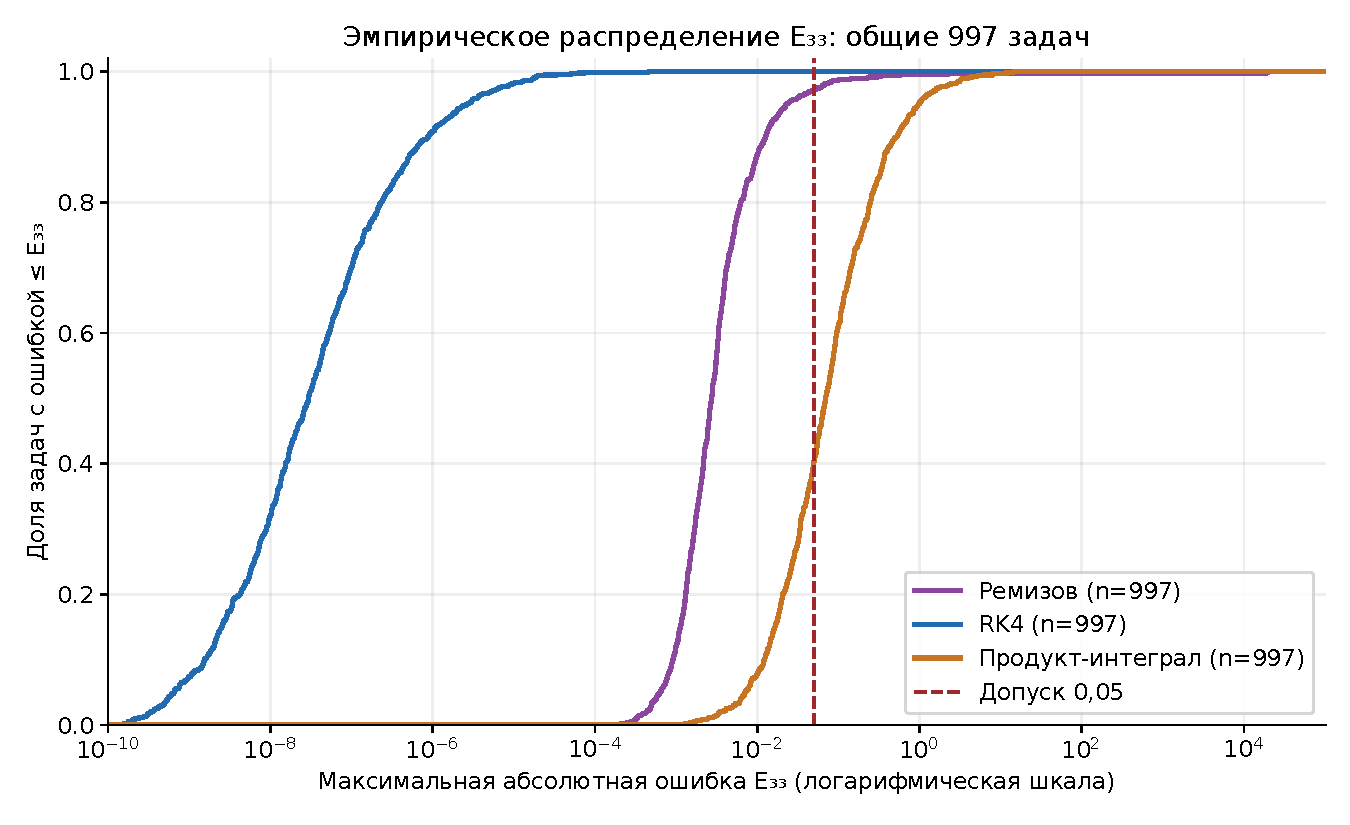
\includegraphics[width=0.95\textwidth]{grid33_supplement/figures/01_ecdf_common997.pdf}
\caption{Общие 997 задач; логарифмическая ось ошибок, линейная накопленная доля. MC не показан, поскольку E33 неизвестна.}
\label{fig:grid33final-1}
\end{figure}

\begin{figure}[!htbp]
\centering
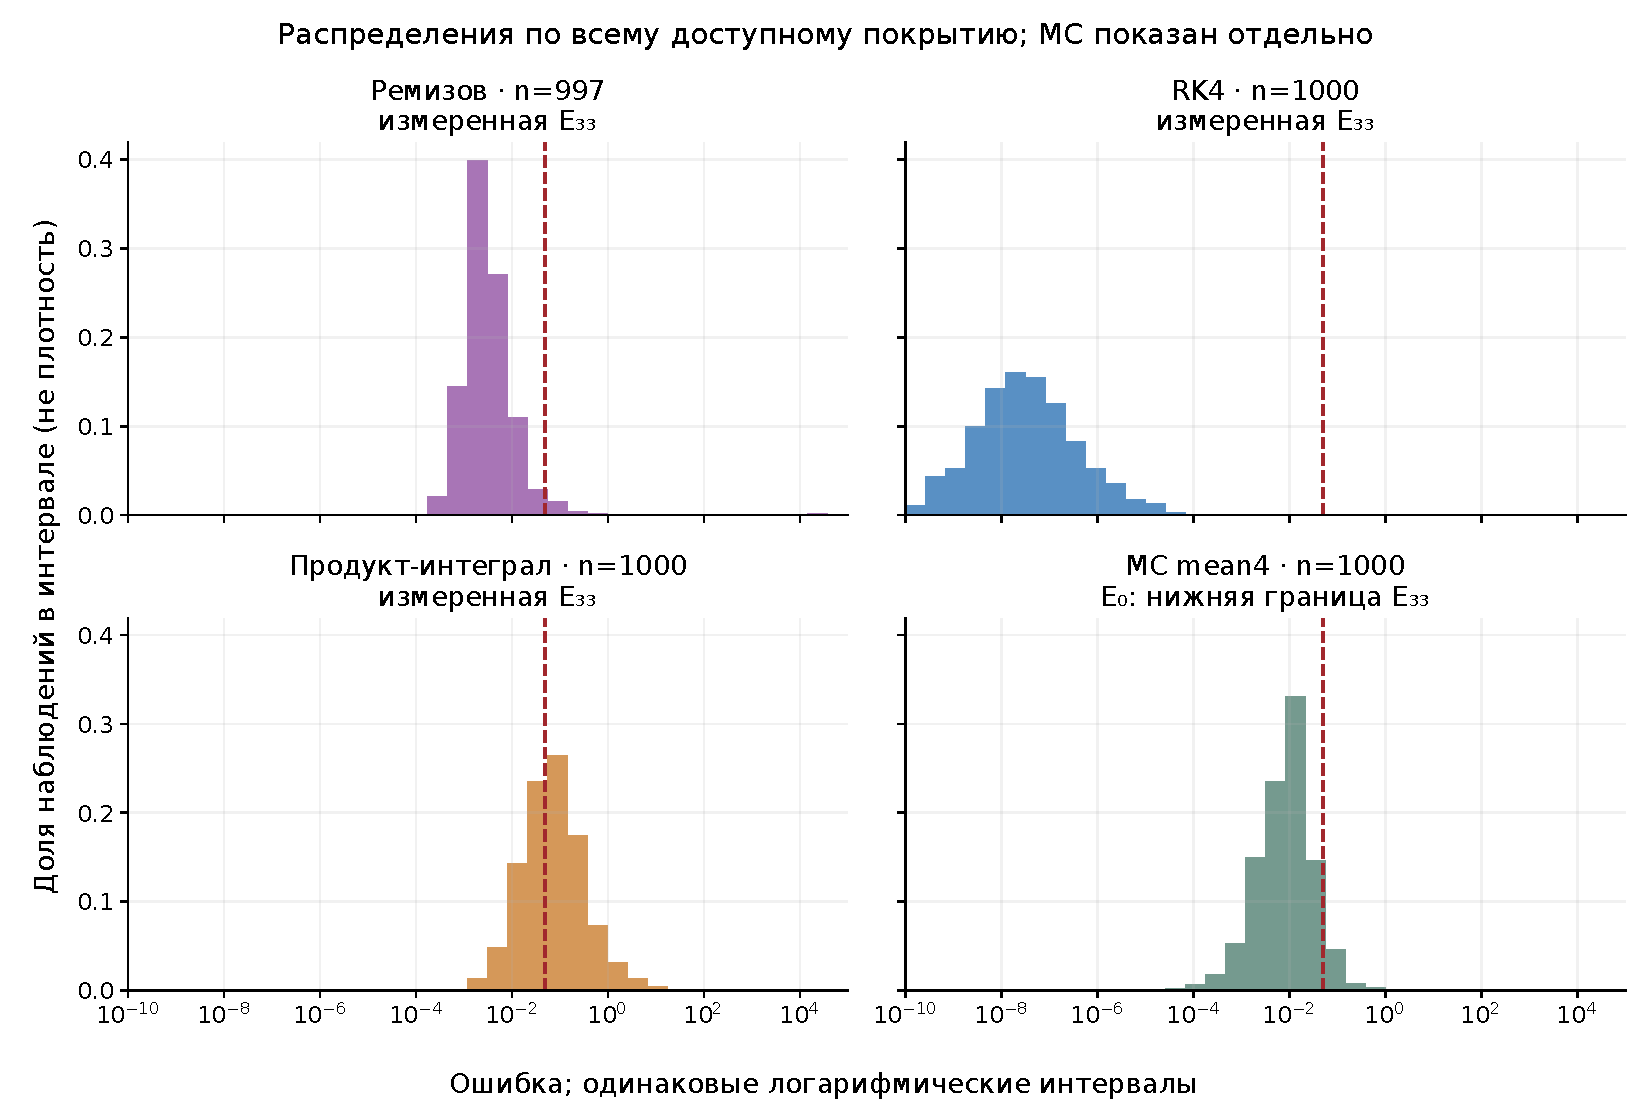
\includegraphics[width=0.95\textwidth]{grid33_supplement/figures/02_histograms_available.pdf}
\caption{Равные интервалы по log10 ошибки, доля в каждом интервале. MC-панель показывает только E0 как нижнюю границу E33; её нельзя читать как распределение MC E33. Все наблюдения сохранены.}
\label{fig:grid33final-2}
\end{figure}

\begin{figure}[!htbp]
\centering
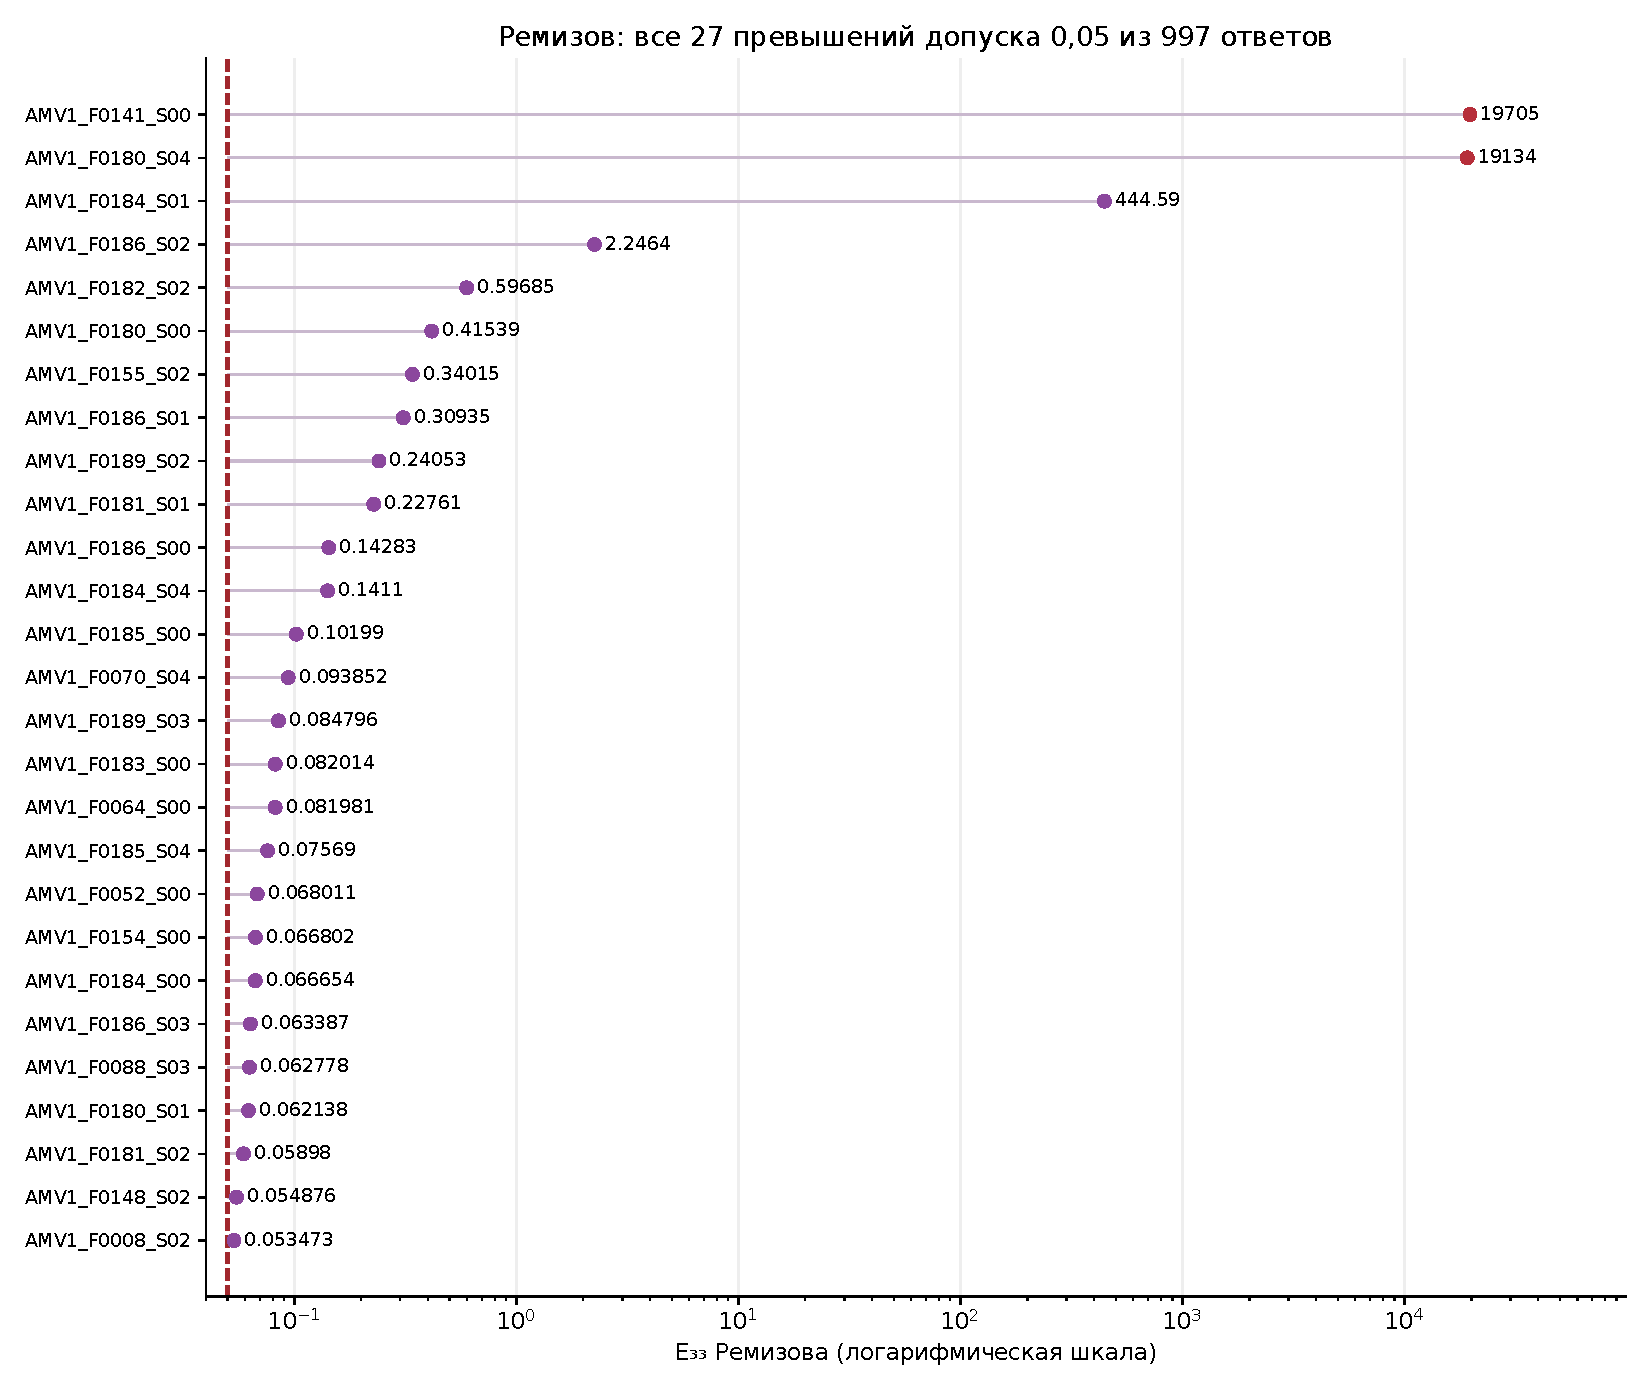
\includegraphics[width=0.95\textwidth]{grid33_supplement/figures/03_remizov_exceedances.pdf}
\caption{Показаны все ответы Ремизова с E33>0,05, без удаления из основных статистик. Два крупнейших выделены цветом; «выброс» здесь описательное слово, не результат статистического теста.}
\label{fig:grid33final-3}
\end{figure}

\begin{figure}[!htbp]
\centering
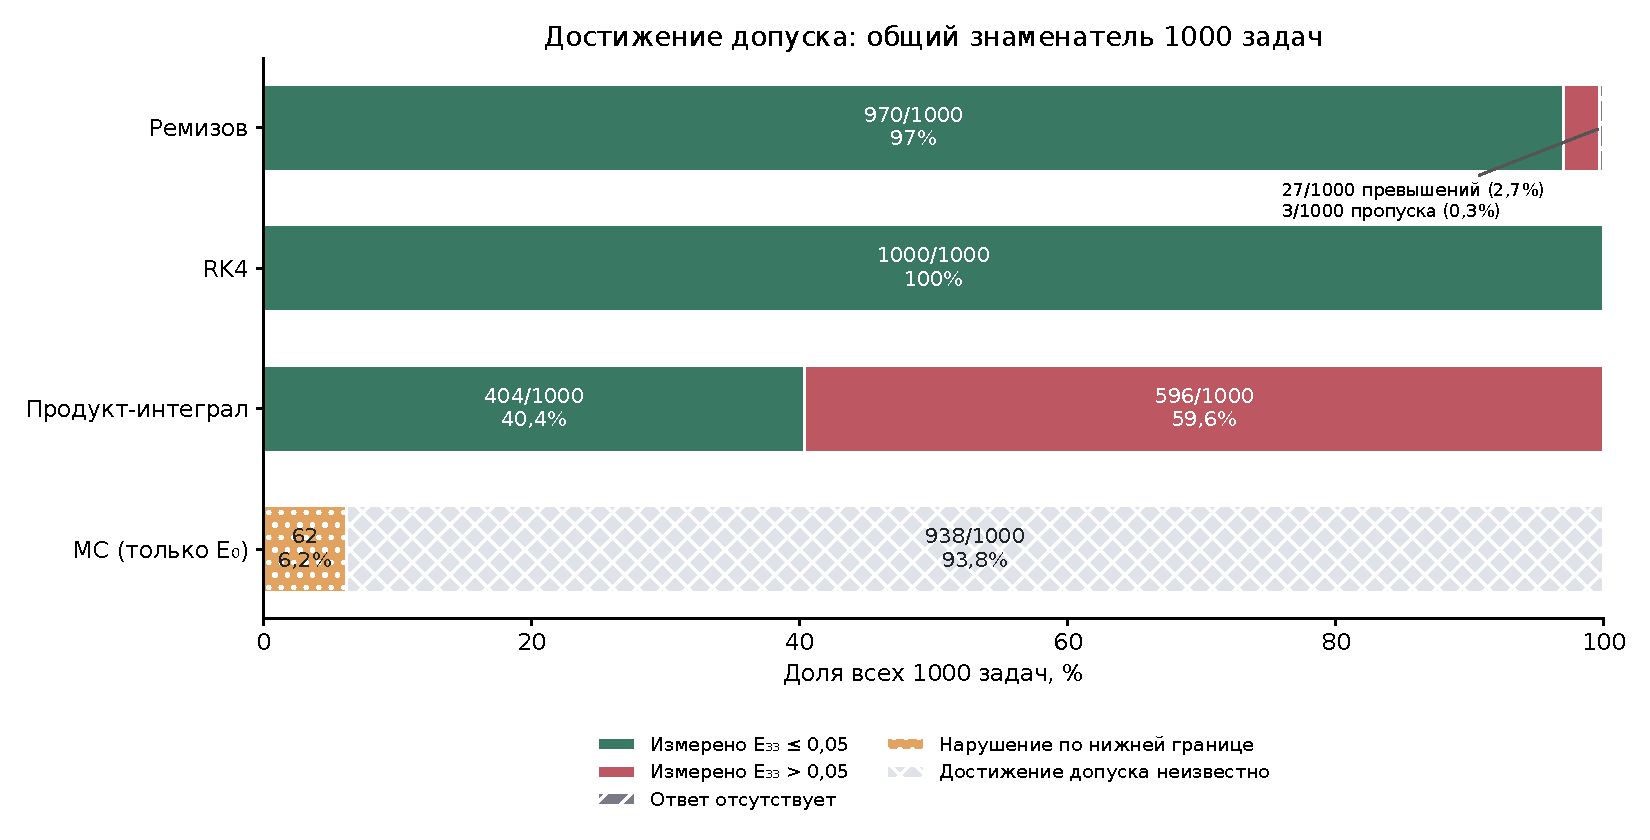
\includegraphics[width=0.95\textwidth]{grid33_supplement/figures/04_threshold_shares.pdf}
\caption{Доли от всех 1000 задач: пропуски R не считаются численными нарушениями. У MC нет измерений E33: 62 нарушения следуют из E0, для 938 достижение допуска неизвестно; условие — тот же ответ MC в нуле.}
\label{fig:grid33final-4}
\end{figure}

\paragraph{Интерпретация и ограничения.}
RK4 имеет наименьшую измеренную ошибку при данном бюджете и точных НУ.
Это не доказательство порядка или скорости сходимости: контрольная сетка
и параметры не уточнялись. Для такой оценки нужны отдельные серии
как минимум из трёх успешных уровней при контроле остальных параметров.
Малая ошибка в одной конфигурации не устанавливает лучшую стоимость
достижения точности. Уточнение контрольной сетки может диагностировать
пропущенные экстремумы, но само по себе не доказывает непрерывной границы.
Задачи внутри семейства зависимы; доли описывают фиксированный набор,
а не доверительные оценки для 1000 независимых наблюдений.

Исторические ML-метрики относятся к $E_0$ и на $E_{33}$ не переносятся.
На нынешних 997 четырёхметодных метках один класс RK4; обучение такого
селектора не даёт содержательной проверки выбора. Для постановки без
RK4 нужны полные сопоставимые MC33. Независимая генерализация на новые
семейства, другие бюджеты, неточные НУ и иной класс ОДУ не установлена.

\paragraph{Выводы и оставшиеся требования.}
Сохранённые массивы позволяют без повторного решения получить E33
для R/RK4/PI и условно доказать строгую победу RK4 на общих 997 задачах.
Три отсутствующих R-ответа, полная MC33, непрерывная норма и сходимость
остаются открытыми. Универсальное превосходство RK4 не утверждается.
Историческое требование выбора быстрейшего надёжного метода при
$E_{\mathrm{grid}}\le0.01$ не закрывается серией с $\varepsilon=0.05$
без сопоставимых времён. Подробный реестр доказательств и требуемых
экспериментов вынесен в сопровождающий файл \texttt{REQUIREMENTS.md}.
Источники: сохранённая CSV \texttt{saved\_grid33\_1000\_2026-11-04},
её независимая проверка и исходный научный отчёт. Новых solver/MC/ML: 0.
